On peut poursuivre la dernière analogie (avec un ordinateur) de la manière suivante. Sur un PC classique, on crée et utilise des applications qui reposent sur un système d'exploitation responsable des éléments matériels. C'est la même chose dans un modèle SDN : on souhaite créer des applications "réseau" sans se soucier de la manière dont les éléments de ce dernier vont s'organiser pour répondre à la problématique. On sépare ainsi la couche applicative, le système d'exploitation réseau et la communication entre les entités du réseau.\\

Pour réaliser cela, il est nécessaire, puisqu'un réseau est constitué d'entités physiquement séparées, de disposer d'un protocole de communication standard entre celles-ci. Mais ça n'est pas suffisant : si tous les éléments communiquent entre eux, encore faut-il qu'ils aient des choses à se dire pour faire circuler, outre les données à faire transiter, les instructions qui vont leur indiquer quoi faire avec ces données. Cela n'est possible que si il existe un cerveau central qui coordonne les opérations (il n'existe pas vraiment d'intelligence collective à ce jour). C'est le rôle du contrôleur SDN. On déporte ainsi l'intelligence humaine déployée dans la configuration de tous les éléments du réseau vers un seul (même si il peut être dupliqué).\\



\begin{figure}[h]
  	\centering
  	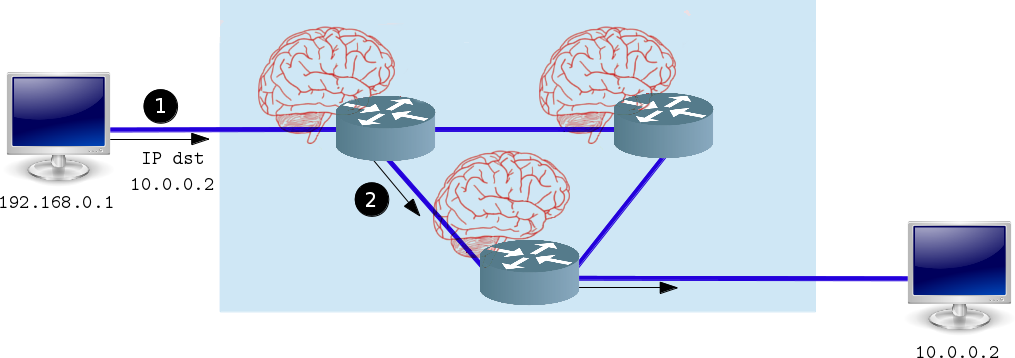
\includegraphics[width=0.85\textwidth]{routage_normal.png}
  	\caption{Réseau classique : chaque routeur contient une partie de la logique de contrôle}
\end{figure}

\begin{figure}[h]
  	\centering
  	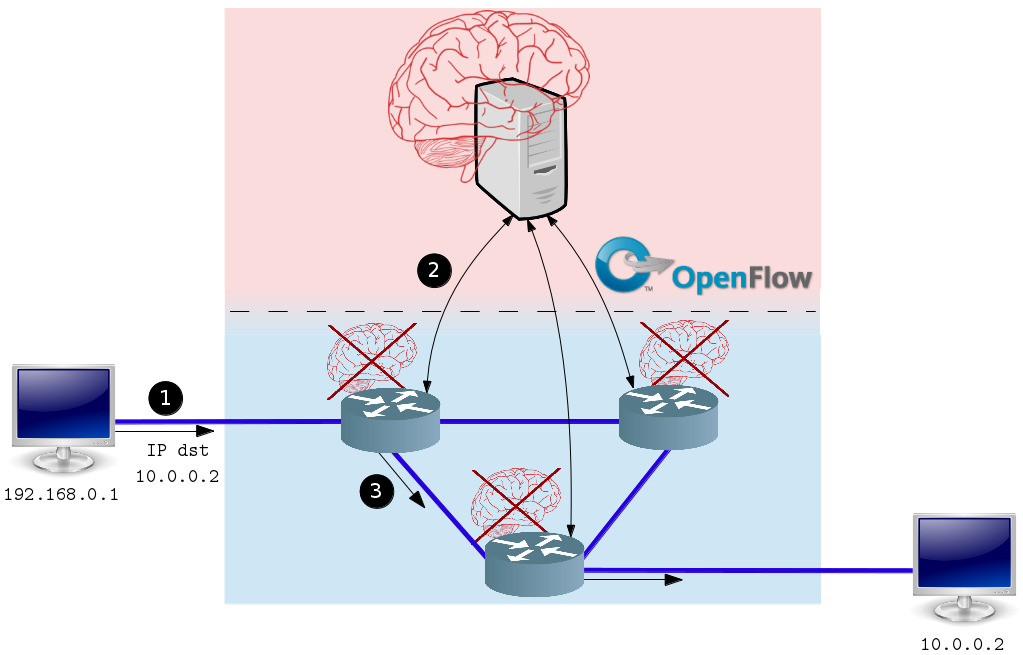
\includegraphics[width=0.8\textwidth]{openflow.png}
  	\caption[Caption for LOF]{Réseau SDN : "l'intelligence" est déportée vers le contôleur \footnotemark}
\end{figure}

\footnotetext{\label{rapport_maxence} Schéma extrait du mémoire "Étude d’OpenFlow dans le contexte de la sécurité" de Maxence Tury}

Les avantages de cette architecture sont multiples :
\begin{list}{$\Autumntree$}{}
\item D'abord cela réduit grandement la complexité de configuration manuelle et le risque d'erreur (si le système d'exploitation réseau est fiable).
\item Cela facilite donc énormément le développement d'applications réseau complexes, puisque la tâche peut être quasiment séparée de sa réalisation physique.
\item Les routes optimales sont plus facilement calculables qu'au sein d'un réseau classique : un seul élément gère les différentes distances et métriques qui peuvent changer selon le trafic, et être modifiées à la volée par des applications spécifiques.
\item La gestion du réseau devient plus simple, les évènements importants (perte d'un lien, disfonctionnement, ralentissement ...) peuvent être remarqués rapidement, la réaction pouvant être automatique et quasiment instantanée.
\item Les coûts matériels sont diminués puisque seuls subsistent les switchs "de base" et le contrôleur qui n'est pas réellement un équipement spécifique. Le reste peut être pris en charge logiciellement au niveau du contrôleur.
\end{list}

Bref, pour résumer, beaucoup plus de flexibilité est permise par cette approche, économisant temps et matériel. Evidemment, l'idée n'est pas nouvelle, mais n'a pas que des avantages. Notamment : la sécurité du contrôleur devient un point brûlant, puisque toute la gestion du réseau provient de lui.